% Enable warnings about problematic code
\RequirePackage[l2tabu, orthodox]{nag}

\documentclass{WeSTassignment}
\usepackage{minted}
\usepackage{graphicx}

% The lecture title, e.g. "Web Information Retrieval".
\lecture{Introduction to Web Science}
% The names of the lecturer and the instructor(s)
\author{%
  Prof. Dr.~Steffen~Staab\\{\normalsize\mailto{staab@uni-koblenz.de}} \and
  Ren{\'e}~Pickhardt\\{\normalsize\mailto{rpickhardt@uni-koblenz.de}} \and
   Korok~Sengupta\\{\normalsize\mailto{koroksengupta@uni-koblenz.de}}
}
% Assignment number.
\assignmentnumber{2}
% Institute of lecture.
\institute{%
  Group Tango\\%
  Institute of Web Science and Technologies\\%
  Department of Computer Science\\%
  University of Koblenz-Landau%
}
% Date until students should submit their solutions.
\datesubmission{November 9, 2016, 10:00 a.m.}
% Date on which the assignments will be discussed in the tutorial.
\datetutorial{November 11th, 2016, 12:00 p.m.}



\author{%
  Mariya Chkalova \\{\normalsize\mailto{mchkalova@uni-koblenz.de}} \and
  Arsenii Smyrnov\\{\normalsize\mailto{smyrnov@uni-koblenz.de}} \and
   Simon Schauß\\{\normalsize\mailto{sschauss@uni-koblenz.de}}
}


% Set langauge of text.
\setdefaultlanguage[
  variant = american, % Use American instead of Britsh English.
]{english}

% Specify bib file location.
\addbibresource{bibliography.bib}

% For left aligned centerd boxes
% see http://tex.stackexchange.com/a/25591/75225
\usepackage{varwidth}

% ==============================================================================
% Document

\begin{document}

\maketitle

The main objective of this assignment is for you to use different tools with which you can understand the network that you are connected to or you are connecting to in a better sense.
These tasks are not always specific to \enquote{Introduction to Web Science}.
For all the assignment questions that require you to write a code, make sure to include the code in the answer sheet, along with a separate python file. Where screen shots are required, please add them in the answers directly and not as separate files. 





% ------------------------------------------------------------------------------

\section{IP Packet (5 Points)}

Consider the IPv4 packet that is received as:\\ \\
\texttt{4500 062A 42A1 8001 4210 XXXX C0A8 0001 C0A8 0003}\\ \\ 
Consider \texttt{XXXX} to be the check sum field that needs to be sent with the packet.

Please provide a step-by-step process for calculating the "Check Sum".\\ \\ 

\iffalse
\begin{enumerate}
\item ’45’ corresponds to the first two fields in the header ie  ‘4’ corresponds to the IP version and ‘5’ corresponds to the header length. Since header length is described in 4 byte words so actual header length comes out to be 5×4=20 bytes.
\item ’00’ corresponds to TOS or the type of service. This value of TOS indicated normal operation.
\item ‘062A’ corresponds to total length field of IP header. So in this case the total length of IP packet is 1578.
\item ‘42A1’ corresponds to the identification field.
\item ‘8001’ can be divided into two bytes. These two bytes (divided into 3 bits and 13 bits respectively) correspond to the flags and fragment offset of IP header fields.
\item ‘4210’ can be divided into ’42’ and ’10’. The first byte ’42’ corresponds to the TTL field and the byte ’10’ corresponds to the protocol field of the IP header. ’10’ indicates that the protocol is TCP.
\item ‘xxxx’ corresponds to the checksum which is set at the source end (which sent the packet). .
\item The next set of bytes ‘COA8 0001’ and ‘COA8 0003’ correspond to the source IP address and the destination IP address in the IP header.
\end{enumerate}

1) Convert values to binary:
4500 - 0100 0101 0000 0000
062A - 0000 0110 0010 1010
42A1 - 0100 0010 1010 0001
8001 - 1000 0000 0000 0001
4210 - 0100 0010 0001 0000
C0A8 - 1100 0000 1010 1000
0001 - 0000 0000 0000 0001
C0A8 - 1100 0000 1010 1000
0003 - 0000 0000 0000 0011

2) Add these binary values one by one:
4500 - 0100 0101 0000 0000
062A - 0000 0110 0010 1010
     - 0100 1011 0010 1010 //First result
42A1 - 0100 0010 1010 0001
     - 1000 1101 1100 1011 //Second result
8001 - 1000 0000 0000 0001
     -10000 1101 1100 1100 //One odd bit (carry),  add that odd bit to the result as we need to keep the checksum in 16 bits.
     - 0000 1101 1100 1101 //Third result
4210 - 0100 0010 0001 0000
     - 0100 1111 1101 1101 //Fourth result
c0a8 - 1100 0000 1010 1000
     -10001 0000 1000 0101 //Carry again, add this bit
     - 0001 0000 1000 0110 //Fifth result
0001 - 0000 0000 0000 0001
     - 0001 0000 1000 0111 //Sixth result
c0a8 - 1100 0000 1010 1000
     - 1101 0001 0010 1111 //Seventh result
0003 - 0000 0000 0000 0011
     - 1101 0001 0011 0000 //Final result   
     

Result: 1101 0001 0011 0000
3) Complement the result to obtain checksum in binary format:
0010111011001111 - checksum, that is equal to 2ECF in HEX.
So, checksum is 2ECF.
\fi

Step \textbf{1}:

calculate the sum of each 16bit block

\begin{align*}
+ &  4500  \\
+ &  062A \\
+ &  42A1 \\
+ &  8001 \\
+ &  4210 \\
+ &  C0A8 \\
+ &  0001 \\
+ &  C0A8 \\
+ &  0003 \\
= & 2D130
\end{align*}

Step \textbf{2}:

excerpt the carry bit and calculate the sum:

\begin{align*}
D130 + 2 = D132
\end{align*}

Step \textbf{3}:

build the inverse of each 4bit block in the hexadecimal system

\begin{align*}
D132 \Rightarrow 2ECD
\end{align*}

Therefore the checksum is 2ECD


% ------------------------------------------------------------------------------

\section{Routing Algorithm (10 Points)}
\textbf{UPDATE. The bold fonted numbers have been updated on Monday Nov. 7th. (If you already have done so feel free to use the old numbers. But the solution with the old version will be more complex than the solution with the updated numbers.)}

You have seen how routing tables can be used to see how the packets are transferred across different networks. Using the routing tables below of Router 1, 2 and 3:
\begin{enumerate}
\item Draw the network \texttt{[6 points]}
\item Find the shortest path of sending information from 67.68.2.10 network to 25.30.3.13 network \texttt{[4 points]}
\end{enumerate}

\begin{table}[h]
\centering
\caption{Router 1}
\label{Router 1}
\begin{tabular}{ccc}
\hline
\multicolumn{1}{|c|}{\textbf{Destination}} & \multicolumn{1}{c|}{\textbf{Next Hop}} & \multicolumn{1}{c|}{\textbf{Interface}} \\ \hline
67.0.0.0                                   & 67.68.3.1                              & eth 0                                   \\
62.0.0.0                                   & 62.4.31.7                              & eth 1                                   \\
88.0.0.0                                   & 88.4.32.6                              & eth 2                                    \\
141.\textbf{71}.0.0                                  & 141.\textbf{71}.20.1                            & eth 3                                    \\
26.0.0.0                                   & 141.71.26.3                            & eth 3                                   \\
\textbf{156.3}.0.0                                  & 141.71.26.3                            & eth 3                                   \\
205.\textbf{30.7}.0                                  & 141.71.26.3                            & eth 3                                    \\
25.0.0.0                                   & 88.6.32.1                              & eth 2                                    \\
121.0.0.0                                  & 88.6.32.1                              & eth 2                                   
\end{tabular}
\end{table}
\begin{table}[h]
\centering
\caption{Router 2}
\label{Router 2}
\begin{tabular}{ccc}
\hline
\multicolumn{1}{|c|}{\textbf{Destination}} & \multicolumn{1}{c|}{\textbf{Next Hop}} & \multicolumn{1}{c|}{\textbf{Interface}} \\ \hline
141.\textbf{71}.0.0                                  & 141.71.26.3                            & eth 3                                   \\
205.\textbf{30.7}.0                                  & 205.\textbf{30.7}.1                            & eth 0                                   \\
26.0.0.0                                   & 26.3.2.1                               & eth 2                                    \\
156.\textbf{3}.0.0                                  & 156.3.0.6                              & eth 1                                   \\
67.0.0.0                                   & 141.\textbf{71}.20.1                            & eth 3                                   \\
62.0.0.0                                   & 141.\textbf{71}.20.1                            & eth 3                                   \\
88.0.0.0                                   & 141.\textbf{71}.20.1                            & eth 3                                    \\
25.0.0.0                                   & 205.30.7.2                             & eth 0                                   \\
121.0.0.0                                  & 205.30.7.2                             & eth 0                                  
\end{tabular}
\end{table}
\begin{table}[h]
\centering
\caption{Router 3}
\label{Router 3}
\begin{tabular}{ccc}
\hline
\multicolumn{1}{|c|}{\textbf{Destination}} & \multicolumn{1}{c|}{\textbf{Next Hop}} & \multicolumn{1}{c|}{\textbf{Interface}} \\ \hline
205.\textbf{30.7}.0                                  & 205.30.7.2                             & eth 0                                   \\
88.0.0.0                                   & 88.6.32.1                              & eth 1                                   \\
25.0.0.0                                   & 25.30.1.2                              & eth 2                                   \\
121.0.0.0                                  & 121.0.3.1                              & eth 3                                   \\
156.\textbf{3}.0.0                                  & 205.\textbf{30}.7.1                             & eth 0                                   \\
26.0.0.0                                   & 205.\textbf{30}.7.1                             & eth 0                                   \\
141.0.0.0                                  & 205.\textbf{30}.7.1                             & eth 0                                   \\
67.0.0.0                                   & 88.4.32.6                              & eth 1                                   \\
62.0.0.0                                   & 88.4.32.6                              & eth 1                                  
\end{tabular}
\end{table}


% ------------------------------------------------------------------------------
\subsection*{1.}
\begin{figure}[ht!]
\centering
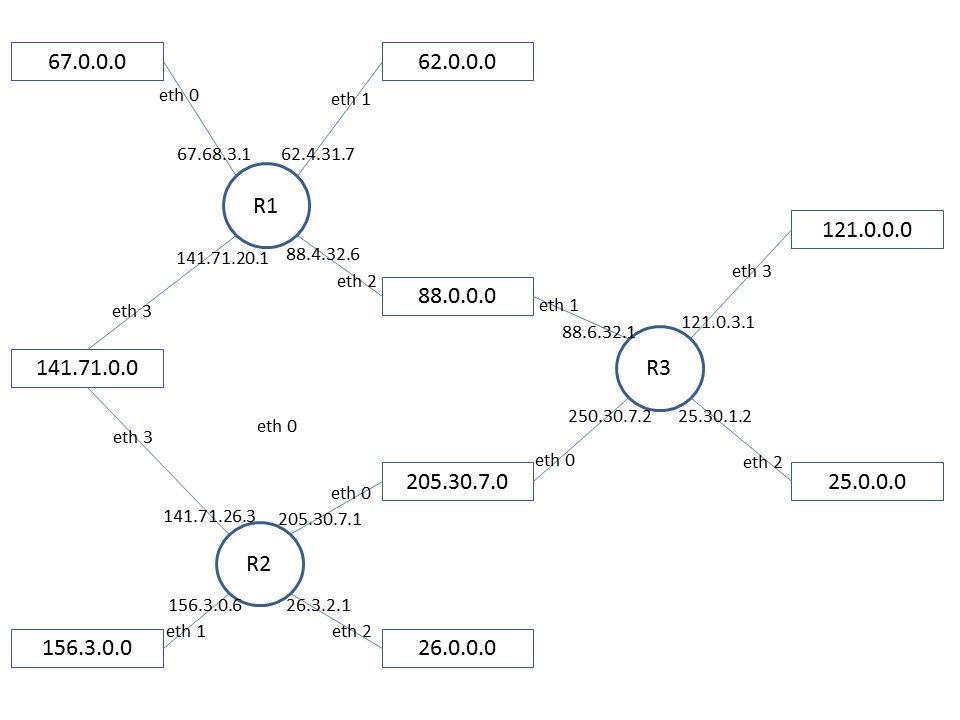
\includegraphics[width=\textwidth]{tango_assignment2_2_2.jpg}
\caption{Network \label{overflow}}
\end{figure}

See: \ref{overflow}

% ------------------------------------------------------------------------------
\subsection*{2.}
The shortest path of sending information from 67.68.2.10 network to 25.30.3.13 network:\\ \\
send to Router 1 IP=67.68.3.1;\\ \\
Router 1 will forward package to Router 2 IP=88.6.32.1\\ \\
Router 2 will deliver package via 25.0.0.0 network to the destination computer.\\ \\

% ------------------------------------------------------------------------------



\section{Sliding Window Protocol (10 Points)}
\emph{Sliding window algorithm, which allows a sender to have more than one unacknowledged packet "in flight" at a time, improves network throughput. }\\ \\
Let us consider you have 2 Wide Area Networks. One with a bandwidth of 10 Mbps (Delay of 20 ms) and the other with 1 Mbps (Delay of 30 ms) . If a packet is considered to be of size 10kb. Calculate the window size of number of packets necessary for Sliding Window Protocol. [\texttt{5 points}]\\
\textbf{Answer:} \\
WAN1 Window size: (2 * 10 Mb/s * 0.02s)/10 Kb = 40 \\
WAN2 Window size: (2 * 1 Mb/s * 0.03s)/10 Kb = 6 


Since you now understand the concept of Window Size for Sliding Window Protocol and how to calculate it, consider a window size of 3 packets and you have 7 packets to send. Draw the process of \texttt{Selective Repeat Sliding Window Protocol} where in the 3rd packet from the sender is lost while transmission. Show diagrammatically how the system reacts when a packet is not received and how it recuperates from that scenario. [\texttt{5 points}]\\ 
\textbf{Answer:} \\
\begin{figure}[ht]
	\centering
	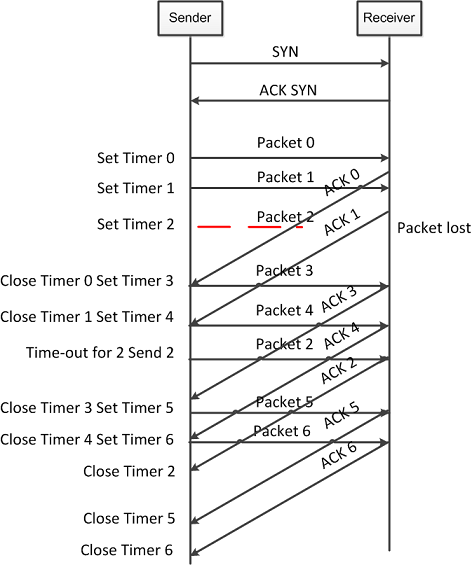
\includegraphics[width=0.9\textwidth]{tango_assignment2_3_2.png}
	\caption{Packet loss}
	\label{fig:packet_loss}
\end{figure}


In Selective-Repeat ARQ, the receiver while keeping track of sequence numbers, buffers the frames in memory and sends NACK for only frame which is missing or damaged.
The sender in this case, sends only packet for which NACK is received.



% ------------------------------------------------------------------------------

\section{TCP Client Server (10 Points)}

Use the information from the \href{https://docs.python.org/3/howto/sockets.html}{socket} documentation and create: [\texttt{4 points}]
\begin{enumerate}
\item a simple TCP Server that listens to a
\item Client
\end{enumerate}
\underline{Note:} Please use port \texttt{8080} for communication on \texttt{localhost} for client server communication.\\ \\
Given below are the following points that your client and server must perform: [\texttt{6 points}]
\begin{enumerate}
\item The \emph{Client} side asks the user to input their name, age \& \emph{matrikelnummer} which is then sent to the server all together.
\item Develop a protocol for sending these three information and subsequently receiving each of the information in three different lines as mentioned in the below format. Provide reasons for the protocol you implemented. 
\item Format the output in a readable format as:\texttt{\\ Name: Korok Sengupta; \\ Age: 29; \\ Matrikelnummer: 21223ert56}
\end{enumerate}

Provide a snapshot of the results along with the code. \\

\begin{listing}
	\centering
	\inputminted{python}{tango_assignment2_4_client.py}
    \caption{TCP client}
\end{listing}

\begin{listing}
	\centering
	\inputminted{python}{tango_assignment2_4_server.py}
    \caption{TCP server}
\end{listing}


\begin{figure}[ht]
	\centering
	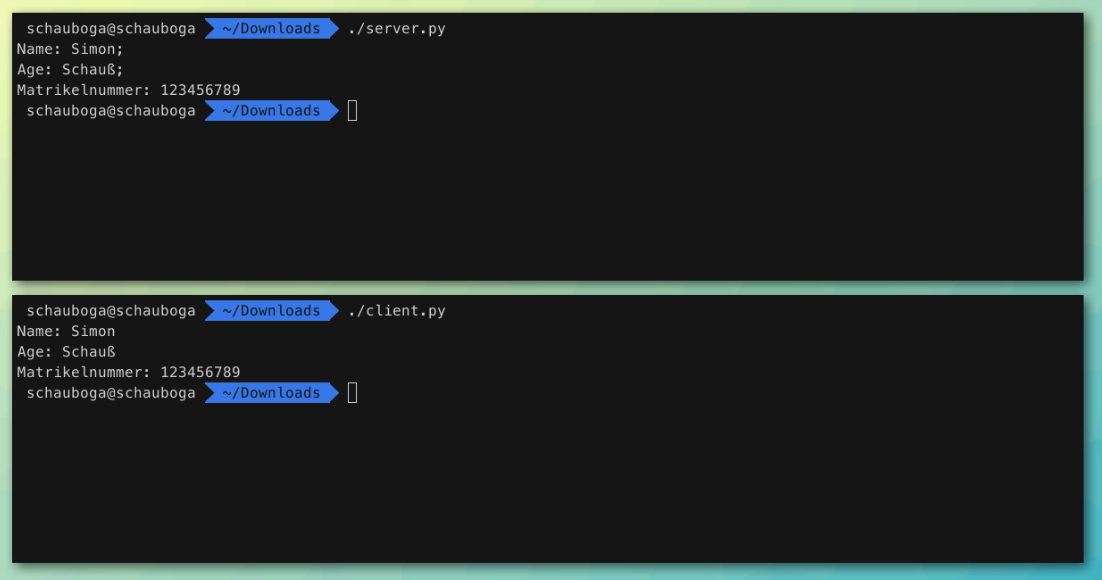
\includegraphics[width=0.9\textwidth]{tango_assignment2_4.png}
	\caption{TCP client/server in action}
	\label{fig:tcp_server}
\end{figure}



\makefooter

\end{document}
